\documentclass[11pt,a4paper]{article}
\usepackage[T1]{fontenc}
\usepackage[margin=2.3cm]{geometry}
\usepackage{amsmath,amssymb}
\usepackage{graphicx}
\usepackage[dvipsnames]{xcolor}
\usepackage{enumitem}
\usepackage[colorlinks=true,linkcolor=blue,urlcolor=blue]{hyperref}
\setlength{\parskip}{0.6em}
\setlength{\parindent}{0pt}
\begin{document}

\begin{center}{\LARGE\bfseries openunits}\\[0.4em]{\large Catch the Mars Climate Orbiter units bug before it flies, in three sessions.}\\[0.2em]\small PAN IIT OSS explainer \textbullet{} secondary school to diploma / undergraduate (levels 3-5)\end{center}

\section*{Why this exists}
Every measurement is a number and a unit, and every calculation must respect both. This explainer shows how to convert units, check equations by their dimensions and see how a unit mistake grows, using only arithmetic and a little numpy.

\section*{The end goal}
Catch the Mars Climate Orbiter units bug before it flies. The end goal is to catch a units bug like the one behind the loss of the Mars Climate Orbiter in 1999 before it flies: attach units to every number, check dimensions, and test the whole chain on a toy trajectory.

\section*{How the three sessions build up}
\begin{enumerate}[nosep]
\item \textbf{Session 1: A number without a unit is not an answer} (Level 1, conceptual interactive model, 60 min).
\item \textbf{Session 2: Dimensional analysis and the growth of unit errors} (Level 2, mathematical engineering model, 75 min).
\item \textbf{Session 3: A toy trajectory and a units-checked wrapper} (Level 3, simulation and validation, 90 min).
\end{enumerate}

\section{Session 1: A number without a unit is not an answer}

\subsection*{A. Real-world problem}
A friend texts 'the car did 60'. Sixty what? Metres per second is a fast sprinter, kilometres per hour is a slow city drive, miles per hour is a little faster than that. Mixing units is not just a school mistake: it has cost real engineering projects dearly. Can we build a converter that never forgets the unit, and see how much a missing unit can change a number?

\subsection*{B. Concept and theory}
SI (the international system of units) uses the metre (m) for length, the kilogram (kg) for mass and the second (s) for time. Every other unit is a fixed multiple of an SI unit: 1 km = 1000 m, 1 ft = 0.3048 m and 1 mile = 1609.344 m exactly. To convert, change to SI and then to the target unit: the number in the new unit is the old number times (size of old unit) divided by (size of new unit). A prefix is a power of ten written in front of a unit: kilo = 10\textasciicircum{}3, milli = 10\textasciicircum{}-3, micro = 10\textasciicircum{}-6. Significant figures say how many digits of a number you can trust: a result should not claim more digits than the input data.

\begin{itemize}[nosep]
\item n: the number written before the unit (no unit)
\item F\_u: size of unit u in SI (SI units per unit)
\item v: a speed (m/s)
\item k: power of ten of a prefix (no unit)
\end{itemize}

\begin{equation*}
n_{\text{new}}=n_{\text{old}}\,\frac{F_{\text{old}}}{F_{\text{new}}}
\end{equation*}

\begin{equation*}
1\ \text{km/h}=\frac{1000\ \text{m}}{3600\ \text{s}}=0.2778\ \text{m/s}
\end{equation*}

\begin{equation*}
\text{kilo}=10^{3},\qquad \text{milli}=10^{-3},\qquad \text{micro}=10^{-6}
\end{equation*}

\begin{center}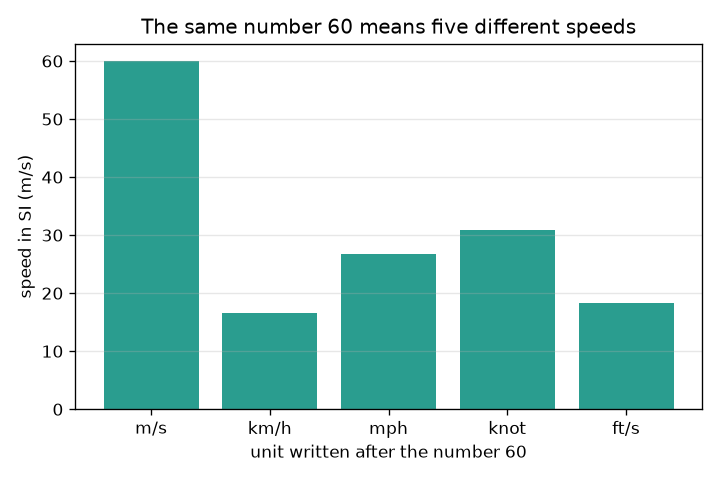
\includegraphics[width=0.85\linewidth]{figures/s01_same_number.png}\\\small The number 60 with five different units means five different speeds.\end{center}

\subsection*{E. Worked example}
A sign says 72 km/h. Find the speed in m/s. Then convert 60 mph to km/h and give the answer to 3 significant figures.
\begin{enumerate}[nosep]
\item 1 km/h = 1000 m / 3600 s = 0.27778 m/s.
\item 72 km/h = 72 * 0.27778 = 20.0 m/s.
\item 1 mph = 1609.344 m / 3600 s = 0.44704 m/s, and 1 km/h = 0.27778 m/s.
\item 60 mph = 60 * 0.44704 / 0.27778 = 96.56 km/h.
\item To 3 significant figures: 96.6 km/h.
\end{enumerate}
\textbf{Answer.} 72 km/h is exactly 20 m/s, and 60 mph is 96.6 km/h (3 significant figures).

\subsection*{F. Questions}
\begin{enumerate}[nosep]
\item \textbf{Conceptual.} Why is '60' not a complete answer to 'how fast was the car?' What must you add, and why does the SI unit help when two people disagree?
\item \textbf{Numerical.} Convert 100 km/h to m/s and to mph. Check that your answers are sensible.
\item \textbf{Graph and simulation interpretation.} In the graph of speed against the number read, which unit gives the highest speed for the number 60, and which the lowest? What does the slope of each line mean?
\item \textbf{Design and optimisation challenge.} Design: a road sign for visitors must show a 50 km/h limit and a mph equivalent. Choose a rounding and justify it, noting the trade-off between clarity and accuracy.
\end{enumerate}

\section{Session 2: Dimensional analysis and the growth of unit errors}

\subsection*{A. Real-world problem}
An engineer writes s = u t + a t. A student feeds a pipe length in feet into a formula built for metres. Neither mistake is caught by the computer, because a computer only sees numbers. Can we check a formula by looking only at the kinds of quantity in it, and can we say how bad a unit mistake will be before it happens?

\subsection*{B. Concept and theory}
Every physical quantity has a dimension: a combination of the base dimensions mass (M), length (L) and time (T). Write it as an exponent vector [M, L, T]. A speed is length over time, [0, 1, -1]; a force is mass times acceleration, [1, 1, -2]. Multiplying quantities adds their vectors; dividing subtracts; raising to a power multiplies. An equation is dimensionally consistent only if every term that is added has the same vector as the left side. If the dimensions fail to match, the equation is certainly wrong; if they match, it may still be wrong (for example a missing factor of 1/2). If a quantity depends on others through a product of powers, matching the exponents gives linear equations for the powers. Finally, if a length unit is wrong by a factor f, a quantity of dimension L\textasciicircum{}b is wrong by f\textasciicircum{}b.

\begin{itemize}[nosep]
\item M, L, T: base dimensions: mass, length, time (exponents (no unit))
\item d: dimension vector [M, L, T] (exponents)
\item f: factor by which a length is mis-scaled (no unit)
\item g: gravitational acceleration (9.80665) (m/s\textasciicircum{}2)
\item e\_i: relative error of input i (no unit)
\end{itemize}

\begin{equation*}
[\text{force}]=\mathsf{M}\,\mathsf{L}\,\mathsf{T}^{-2},\qquad [\text{impulse}]=[\text{force}][\text{time}]=\mathsf{M}\,\mathsf{L}\,\mathsf{T}^{-1}
\end{equation*}

\begin{equation*}
T\propto L^{p}g^{q}m^{r}:\quad r=0,\ \ p+q=0,\ \ -2q=1\ \Rightarrow\ T\propto\sqrt{L/g}
\end{equation*}

\begin{equation*}
\text{error factor}=f^{\,b}\ \text{for a quantity of dimension }\mathsf{L}^{b}
\end{equation*}

\begin{equation*}
\frac{\delta Q}{Q}\approx\sqrt{\sum_i\left(n_i\,e_i\right)^2}\ \text{ for }Q=\prod_i x_i^{n_i}
\end{equation*}

\begin{center}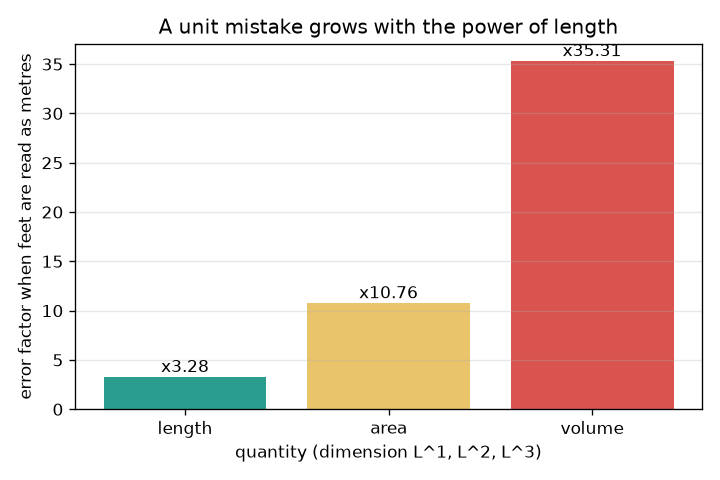
\includegraphics[width=0.85\linewidth]{figures/s02_error_factors.png}\\\small Feet read as metres: the error grows with the power of length in the dimension.\end{center}

\subsection*{E. Worked example}
Use dimensions to find how the period T of a pendulum depends on its length L, on g and on its mass m, then compute the period for L = 1.000 m.
\begin{enumerate}[nosep]
\item Assume T \textasciitilde{} L\textasciicircum{}p g\textasciicircum{}q m\textasciicircum{}r. Dimensions: L is [0, 1, 0], g is [0, 1, -2], m is [1, 0, 0], T is [0, 0, 1].
\item Mass exponent: r = 0, so the mass does not matter.
\item Length exponent: p + q = 0. Time exponent: -2q = 1, so q = -0.5 and p = 0.5.
\item So T = (constant) * sqrt(L/g). The constant is not fixed by dimensions; physics gives 2 pi for small swings.
\item For L = 1.000 m and g = 9.80665 m/s\textasciicircum{}2: T = 2 pi sqrt(1/9.80665) = 2.006 s.
\end{enumerate}
\textbf{Answer.} T goes as L\textasciicircum{}0.5 g\textasciicircum{}-0.5 and is independent of mass; a 1.000 m pendulum swings in 2.006 s.

\subsection*{F. Questions}
\begin{enumerate}[nosep]
\item \textbf{Conceptual.} A formula passes the dimension check. Does that prove it is correct? Give an example and say what a failing check proves.
\item \textbf{Numerical.} A tank volume of 12.0 'cubic metres' was really 12.0 cubic feet. By what factor is the volume overstated, and what is the true volume in litres?
\item \textbf{Graph and simulation interpretation.} In the app with p = 1 and q = -1, what dimension does the formula 2 pi L\textasciicircum{}p g\textasciicircum{}q have, and why is the curve far from the grey period curve?
\item \textbf{Design and optimisation challenge.} Design: a mass m on a spring of stiffness k (force per length) oscillates with period T. Use dimensions to find how T depends on m and k, then say what dimensional analysis cannot tell you.
\end{enumerate}

\section{Session 3: A toy trajectory and a units-checked wrapper}

\subsection*{A. Real-world problem}
In 1999 NASA's Mars Climate Orbiter was lost at Mars. The investigation found that ground software produced thruster impulse data in pound-force seconds while the navigation software expected newton seconds. One pound-force second is about 4.45 newton seconds, so the small thruster firings were misjudged by that factor, and the spacecraft approached Mars lower than planned. Could a few lines of code have caught this? This session builds a toy model, not the real mission: its numbers (mass, firings, cruise time) are illustrative and no real mission data are used.

\subsection*{B. Concept and theory}
A thruster firing gives the spacecraft an impulse J (newton seconds). The velocity change is dv = J / m. A sideways kick at time t\_k then makes the spacecraft drift sideways by dv * (t - t\_k) after time t, so with several firings the offset is the sum over firings. Suppose the file lists numbers in lbf*s. The right conversion multiplies the number by 4.448222 to get N*s. If software reads the number as N*s (factor 1) it predicts a push that is 4.448222 times too small, and the actual path drifts away from the predicted one. The miss at the end is therefore (f\_true - f\_used) / m times the sum of J * (T - t\_k). A units-checked wrapper stores values in SI together with a dimension vector; it refuses to add quantities of different dimensions and refuses bare numbers at a boundary. Note that lbf*s and N*s have the same dimension, so only the attached unit and its automatic conversion prevent the mistake, not the dimension check alone.

\begin{itemize}[nosep]
\item J: impulse number in the file for one firing (lbf*s)
\item f: newton seconds per file unit (4.448222 true, 1 for the bug) (N*s per lbf*s)
\item m: spacecraft mass (toy value 600) (kg)
\item dv: velocity change per firing (m/s)
\item t\_k, T: time of firing k and end of cruise (s)
\item n: number of firings (no unit)
\end{itemize}

\begin{equation*}
\Delta v=\frac{J\,f}{m}
\end{equation*}

\begin{equation*}
y(t)=\sum_{k}\Delta v\,(t-t_k)\quad (t\ge t_k)
\end{equation*}

\begin{equation*}
\text{miss}=\frac{n\,J\,(f_{\text{true}}-f_{\text{used}})}{m}\,\bigl(T-\overline{t_k}\bigr),\qquad f_{\text{true}}=4.448222
\end{equation*}

\begin{center}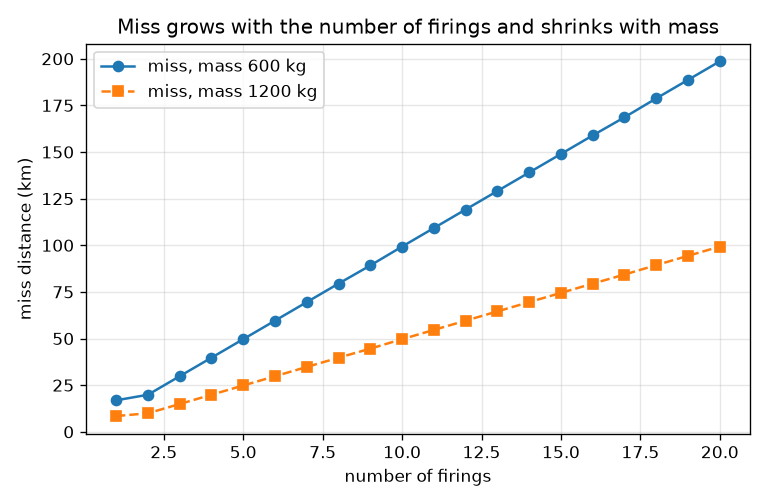
\includegraphics[width=0.85\linewidth]{figures/s03_miss_sensitivity.png}\\\small Miss against number of firings for 600 kg and 1200 kg spacecraft.\end{center}

\subsection*{E. Worked example}
A 600 kg toy spacecraft makes 12 firings of 0.2 lbf*s on days 10, 23, 35, ... 150 (mean day 80). The software reads the numbers as N*s. Find the miss distance at day 180 by hand and compare with the simulation.
\begin{enumerate}[nosep]
\item Mean firing day is 80, so the average drift time is 180 - 80 = 100 days = 8.64 million s.
\item Per firing the true dv is 0.2 * 4.448222 / 600 = 0.0014827 m/s; the predicted dv is 0.2 / 600 = 0.0003333 m/s.
\item Difference per firing: 0.0011494 m/s. For 12 firings: 0.013793 m/s.
\item Miss = 0.013793 m/s * 8.64 million s = 119 170 m = 119.17 km.
\item The simulation gives the same 119.17 km, and the actual path is 4.4482 times the predicted one (153.73 km against 34.56 km).
\end{enumerate}
\textbf{Answer.} Miss of about 119.2 km in the toy model: the real sideways offset is 153.7 km, the predicted one 34.6 km.

\subsection*{F. Questions}
\begin{enumerate}[nosep]
\item \textbf{Conceptual.} Why does a dimension check not catch a lbf*s number read as N*s? What kind of design would catch it?
\item \textbf{Numerical.} Eight firings of 0.5 lbf*s each (on days 10, 30, ... 150) are read as N*s on a 600 kg craft. What is the miss at day 180?
\item \textbf{Graph and simulation interpretation.} In the miss-versus-firings graph, what is the shape of the curve and what does doubling the spacecraft mass do to it?
\item \textbf{Design and optimisation challenge.} Design: with 12 firings of 0.2 lbf*s on a 600 kg craft the miss must stay below 5 km. How wrong may the software's conversion factor be? Propose two checks that would have prevented the bug.
\end{enumerate}

\section{Real-world mini-project}
\textbf{Audit a short engineering calculation for unit errors.} A colleague hands you this four-line calculation for a small thruster test: (1) F = 25 lbf, t = 12 s. (2) Impulse I = F * t = 300. (3) Velocity change dv = I / m with m = 40 kg, so dv = 7.5 m/s. (4) Distance after 1 hour: d = dv * 1 = 7.5 km. Rewrite it with the \texttt{Quantity} class from Session 3, find every unit error, and report the corrected numbers. The colleague also proposes adding a 30 N force to the impulse in a later line: show that the wrapper refuses it.

\section{The path ahead}
\begin{enumerate}[nosep]
\item \textbf{Session 4: Parse compound unit strings.} A parser that builds the dimension and SI size of any compound unit string.
\item \textbf{Session 5: Units at the file boundary.} A reader for small data files with a unit header that converts to SI and refuses files without units.
\item \textbf{Session 6: Carry the uncertainty.} A Quantity that stores a value with an uncertainty and updates it under multiply, divide and power.
\item \textbf{Session 7: A real orbit under gravity.} A planar transfer from Earth's orbit radius (1.496e11 m) to Mars's orbit radius (2.279e11 m) integrated step by step.
\item \textbf{Session 8: Reproduce the Target.} The Target comparison: intended and actual position under gravity, with the distance between them against time.
\end{enumerate}

\section{Answers and hints}

\subsection*{Session 1}
\begin{enumerate}[nosep]
\item \textbf{Conceptual.} Hint: Think about what 60 means with km/h, mph and m/s. Solution: The number alone does not say which unit it counts in; 60 can mean 16.7 m/s, 26.8 m/s or 60 m/s. An answer is a number together with its unit. Converting both to SI (m/s) puts the two statements on the same scale so they can be compared.
\item \textbf{Numerical.} Hint: Use 1 km/h = 0.27778 m/s and 1 mph = 0.44704 m/s. Solution: 100 km/h = 100 / 3.6 = 27.78 m/s. In mph: 27.78 / 0.44704 = 62.14 mph. Sanity check: a mile is longer than a kilometre, so the mph number must be smaller than the km/h number: 62 is smaller than 100. Good.
\item \textbf{Graph and simulation interpretation.} Hint: Compare the heights of the lines at 60 on the x axis. Solution: At 60, m/s gives 60 m/s (highest), mph 26.8 m/s, knot 30.9 m/s, ft/s 18.3 m/s and km/h 16.7 m/s (lowest). The slope is the size of one unit in m/s, so m/s has slope 1 and km/h slope 0.278.
\item \textbf{Design and optimisation challenge.} Hint: Convert 50 km/h to mph and compare rounding up with rounding down. Solution: 50 km/h = 50 * 1000 / 1609.344 = 31.07 mph. Rounding down to 30 mph is easy to read but would let a driver who follows the mph number go 1.07 mph (3.5 percent) too slow, which is safe; rounding up to 31 or 32 invites speeding slightly over the metric limit. A sensible design shows 31 mph (nearest whole number) or states 'about 30 mph' with the legal number in km/h. Assumption: whole numbers are easier to read than decimals.
\end{enumerate}

\subsection*{Session 2}
\begin{enumerate}[nosep]
\item \textbf{Conceptual.} Hint: Compare s = u t + a t\textasciicircum{}2 with the correct version. Solution: No. s = u t + a t\textasciicircum{}2 has all terms with the dimension of length, so it passes, but the correct formula has a factor 1/2 in front of the last term. Dimension checks cannot see pure numbers. A failing check does prove the formula is wrong: s = u t + a t adds a length to a speed.
\item \textbf{Numerical.} Hint: Volume has dimension L\textasciicircum{}3; one foot is 0.3048 m. Solution: The overstatement factor is (1 / 0.3048)\textasciicircum{}3 = 35.31. True volume = 12.0 * 0.3048\textasciicircum{}3 m\textasciicircum{}3 = 12.0 * 0.028317 = 0.340 m\textasciicircum{}3 = 340 litres. Sanity check: a cubic foot is a bit more than 28 litres, and 12 of them are about 340 litres.
\item \textbf{Graph and simulation interpretation.} Hint: Read the readout: the exponent of T is -2q. Solution: The dimension is [0, 0, 2], that is time squared. The value 2 pi L/g at L = 1 m is 0.641 and carries the unit s\textasciicircum{}2, so it cannot be compared with a period in seconds. The dimension view shows the T bar at 2 instead of 1.
\item \textbf{Design and optimisation challenge.} Hint: k has dimension force/length = [1, 0, -2]. Try T \textasciitilde{} m\textasciicircum{}p k\textasciicircum{}q. Solution: Mass exponent: p + q = 0. Time exponent: -2q = 1, so q = -1/2 and p = 1/2, T \textasciitilde{} sqrt(m/k). Length does not appear. Dimensional analysis cannot give the pure number 2 pi, nor tell whether other variables (such as amplitude) matter. Experiment or a real derivation must supply those. Trade-off: speed and generality against exactness.
\end{enumerate}

\subsection*{Session 3}
\begin{enumerate}[nosep]
\item \textbf{Conceptual.} Hint: Compare the dimension vectors of lbf*s and N*s. Solution: Both are force times time, [1, 1, -1], so the dimension check sees no difference; only their size differs (4.448222). A design that attaches the unit to every number (Quantity objects), converts at the boundary and refuses bare numbers would catch it, as would a file format with an explicit unit field.
\item \textbf{Numerical.} Hint: Use the closed form: n J (f\_true - 1) / m times (T - mean firing day). Solution: Mean firing day = 80, so T - mean = 100 days = 8.64e6 s. n J = 4 lbf*s in total. Miss = 4 * 3.448222 / 600 * 8.64e6 = 198 617 m = 198.6 km. Sanity check: it is the same as 20 firings of 0.2 lbf*s, because only n J matters.
\item \textbf{Graph and simulation interpretation.} Hint: Look at the formula: miss is proportional to n and to 1/m (the firing dates also change slightly with n). Solution: The curve is nearly a straight line rising with n (the firing dates move a little as n changes, because they are spread from day 10 to day 150). With mass 1200 kg instead of 600 kg the whole curve is halved: 59.6 km instead of 119.2 km at n = 12, because dv = J f / m.
\item \textbf{Design and optimisation challenge.} Hint: Miss is proportional to \textbar{}4.448222 - f\_used\textbar{}; the case f = 1 gives 119.17 km. Solution: Miss per unit of factor error is 119.17 / 3.448222 = 34.56 km. So \textbar{}4.448222 - f\textbar{} must be below 5 / 34.56 = 0.145: any factor between about 4.30 and 4.59 passes (4.45 gives 0.06 km, 4.4 gives 1.7 km, 4.3 gives 5.1 km). Checks: (1) every file carries a unit field and the reader refuses a file without one; (2) a unit-aware calculation (Quantity) converts to SI at the boundary. A third: an independent end-to-end test with a known thrust.
\end{enumerate}

\section{How to join}
Read \texttt{CONTRIBUTING.md} in the repository, then pick an issue labelled \texttt{good first issue}. Repository: \url{https://github.com/KrunalPanchal1995/openunits}

\end{document}
